\documentclass[
    12pt,
    oneside,
    a4paper,
    chapter=TITLE,
    section=TITLE,
    brazil
]{abntex2}

\usepackage{fontspec}
\usepackage{babel}
\usepackage{graphicx}
\usepackage{microtype}
\usepackage{booktabs}
\usepackage{longtable}
\usepackage{tabularx}
\usepackage{array}
\usepackage{float}
\usepackage{xcolor}
\usepackage{listings}
\usepackage{indentfirst}
\usepackage{url}

\definecolor{ufopblue}{HTML}{1E3A8A}
\definecolor{codebg}{HTML}{F8FAFC}
\definecolor{codeborder}{HTML}{CBD5E1}

\lstdefinelanguage{SQLPostGIS}{
    morekeywords={CREATE, TABLE, EXTENSION, IF, NOT, EXISTS, PRIMARY, KEY, FOREIGN, REFERENCES,
                  CONSTRAINT, CHECK, UNIQUE, NULL, DEFAULT, SERIAL, INTEGER, SMALLINT, BIGINT,
                  VARCHAR, CHAR, NUMERIC, BOOLEAN, GEOMETRY, INDEX, USING, GIST, ON, UPDATE,
                  DELETE, CASCADE, RESTRICT, SELECT, FROM, JOIN, LEFT, WHERE, GROUP, BY, ORDER,
                  DESC, ASC, COUNT, ROUND, SUM, FILTER, AND, OR, IN, AS, UNION, ALL, DISTINCT},
    sensitive=false,
    morecomment=[l]{--},
    morestring=[b]'
}

\lstset{
    language=SQLPostGIS,
    basicstyle=\ttfamily\footnotesize,
    backgroundcolor=\color{codebg},
    frame=single,
    rulecolor=\color{codeborder},
    breaklines=true,
    breakatwhitespace=true,
    tabsize=2,
    showstringspaces=false,
    keywordstyle=\bfseries\color{ufopblue},
    commentstyle=\itshape\color{gray},
    stringstyle=\color{teal}
}

% Informações do trabalho para capa e folha de rosto (abnTeX2)
\titulo{Coleta, Tratamento, Modelagem e Documentação de Base de Dados Geográficos em PostGIS: Infraestrutura Pública e Sistema Viário Regional do Médio Piracicaba (MG)}
\autor{
    Bernardo Martins da Costa Silva (Matrícula: 24.1.8110)\\
    Túlio de Paula Santos Dias (Matrícula: 25.2.8031)
}
\local{João Monlevade -- MG}
\data{2026}
\instituicao{
    Universidade Federal de Ouro Preto -- UFOP\\
    Instituto de Ciências Exatas e Aplicadas -- ICEA\\
    Departamento de Computação e Sistemas -- DECSI
}
\tipotrabalho{Trabalho Acadêmico}
\preambulo{Trabalho apresentado à disciplina \textbf{CSI803 -- Banco de Dados Geográficos}, do curso de Sistemas de Informação do Instituto de Ciências Exatas e Aplicadas da Universidade Federal de Ouro Preto, sob orientação do Prof. Bruno R. Monteiro.}

\hypersetup{
    pdftitle={Base de Dados Geográficos - Médio Piracicaba (MG)},
    pdfauthor={Bernardo Martins da Costa Silva; Túlio de Paula Santos Dias},
    colorlinks=true,
    linkcolor=black,
    citecolor=black,
    urlcolor=ufopblue
}

\setlength{\parindent}{1.25cm}
\setlength{\parskip}{0.2cm}

\begin{document}

\imprimircapa
\imprimirfolhaderosto*

% Resumo
\begin{resumo}
Este trabalho apresenta o processo completo de coleta, tratamento, modelagem espacial, carga em PostgreSQL/PostGIS e documentação de uma base de dados geográficos aberta referente à infraestrutura pública e ao sistema viário regional das Regiões Geográficas Imediatas de João Monlevade e Itabira, em Minas Gerais. A base integra dados oficiais do Instituto Brasileiro de Geografia e Estatística (IBGE) -- limites municipais e população do Censo Demográfico 2022 para 15 municípios -- com feições vetoriais colaborativas do OpenStreetMap obtidas via Overpass API, totalizando 2.179 feições espaciais distribuídas em três camadas geográficas (\texttt{municipio}, \texttt{equipamento\_urbano} e \texttt{trecho\_viario}) e uma tabela de domínio (\texttt{categoria\_equipamento}). Todas as geometrias foram padronizadas no sistema de referência SIRGAS 2000 (EPSG:4674), validadas topologicamente e estruturadas com chaves primárias e estrangeiras, restrições de integridade e índices espaciais GiST. O repositório resultante inclui scripts reproduzíveis de coleta e tratamento em Python, scripts SQL de criação e carga, consultas espaciais de exemplo e dicionário de dados completo.

\vspace{0.4cm}
\noindent\textbf{Palavras-chave:} Banco de Dados Geográficos; PostGIS; Dicionário de Dados; SIRGAS 2000; Médio Piracicaba.
\end{resumo}

\pdfbookmark[0]{\listfigurename}{lof}
\listoffigures*
\cleardoublepage

\pdfbookmark[0]{\listtablename}{lot}
\listoftables*
\cleardoublepage

\pdfbookmark[0]{\contentsname}{toc}
\tableofcontents*
\cleardoublepage

\textual

% ============================================================================
\chapter{Introdução}
% ============================================================================

A organização e a documentação adequadas de bases de dados geográficos constituem etapas fundamentais para garantir a interoperabilidade, a qualidade analítica e a reprodutibilidade de estudos espaciais. Em sistemas gerenciadores de bancos de dados espaciais como o PostgreSQL com a extensão PostGIS, a simples obtenção de arquivos vetoriais brutos não assegura sua usabilidade imediata: é necessário padronizar sistemas de referência de coordenadas, validar geometrias, modelar relacionamentos explícitos e registrar metadados completos em um dicionário de dados.

Neste trabalho, desenvolvido no âmbito da disciplina \textbf{CSI803 -- Banco de Dados Geográficos} da Universidade Federal de Ouro Preto (UFOP), foi construída e documentada a base \texttt{infra\_medio\_piracicaba}, cujo domínio temático abrange a \textbf{infraestrutura pública e o sistema viário regional}. O recorte espacial compreende os \textbf{15 municípios} que integram as Regiões Geográficas Imediatas de João Monlevade (6 municípios) e Itabira (9 municípios), no estado de Minas Gerais, abrangendo aproximadamente 6.099,38~km\textsuperscript{2}.

A escolha do recorte justifica-se tanto pela relevância acadêmica e regional -- por incluir o município sede do Instituto de Ciências Exatas e Aplicadas (ICEA/UFOP) -- quanto pela disponibilidade de dados públicos abertos com licenças compatíveis com redistribuição. O objetivo central é fornecer uma base espacial pronta para importação em um banco PostGIS limpo, acompanhada de documentação autossuficiente que permita a qualquer usuário compreender sua estrutura, limitações e possibilidades analíticas sem necessidade de consultar os autores.

% ============================================================================
\chapter{Fontes de Dados, Licenciamento e Coleta}
% ============================================================================

A construção da base combinou duas fontes públicas amplamente utilizadas em projetos de geoprocessamento no Brasil: o \textbf{IBGE} e o \textbf{OpenStreetMap (OSM)}. Todas as coletas foram automatizadas por meio do script \texttt{scripts/coletar\_dados.py} em \textbf{15/11/2026}, preservando os arquivos originais no diretório \texttt{dados/brutos/}.

\section{Fontes Utilizadas e Licenças}

\begin{enumerate}
    \item \textbf{Instituto Brasileiro de Geografia e Estatística (IBGE):}
    \begin{itemize}
        \item \emph{Conteúdo:} Lista oficial de municípios de Minas Gerais por Região Geográfica Imediata (API de Localidades v1), malhas territoriais em qualidade intermediária (API de Malhas v3, escala de referência 1:250.000) e população residente segundo o Censo Demográfico 2022 (API de Agregados, Agregado 4709, Variável 93).
        \item \emph{URL:} \url{https://servicodados.ibge.gov.br/api/docs} e \url{https://www.ibge.gov.br/geociencias}.
        \item \emph{Licença:} Dados abertos governamentais (Decreto nº 8.777/2016), com atribuição obrigatória da fonte (``Fonte: IBGE'').
    \end{itemize}
    \item \textbf{OpenStreetMap (via Overpass API):}
    \begin{itemize}
        \item \emph{Conteúdo:} Trechos viários estruturantes (\texttt{highway} nas classes \texttt{motorway}, \texttt{trunk}, \texttt{primary}, \texttt{secondary} e \texttt{tertiary}) e equipamentos públicos/comunitários (\texttt{amenity} contemplando estabelecimentos de saúde, ensino, segurança, transporte e serviços públicos).
        \item \emph{URL:} \url{https://www.openstreetmap.org} e \url{https://overpass-api.de}.
        \item \emph{Licença:} \emph{Open Database License} (ODbL 1.0), que permite uso e redistribuição mediante atribuição (``\copyright~OpenStreetMap contributors'') e compartilhamento pela mesma licença.
    \end{itemize}
\end{enumerate}

O código-fonte SQL e os scripts Python do projeto são distribuídos sob a licença MIT, conforme detalhado no arquivo \texttt{LICENSE} do repositório.

\section{Cobertura Espacial e Temporal}

O recorte territorial cobre os seguintes municípios: Bela Vista de Minas, João Monlevade, Nova Era, Rio Piracicaba, São Domingos do Prata e São Gonçalo do Rio Abaixo (Região Imediata de João Monlevade); Bom Jesus do Amparo, Carmésia, Ferros, Itabira, Itambé do Mato Dentro, Passabém, Santa Maria de Itabira, Santo Antônio do Rio Abaixo e São Sebastião do Rio Preto (Região Imediata de Itabira). A Figura~\ref{fig:mapa_recorte} apresenta a distribuição espacial das três camadas tratadas.

\begin{figure}[H]
    \centering
    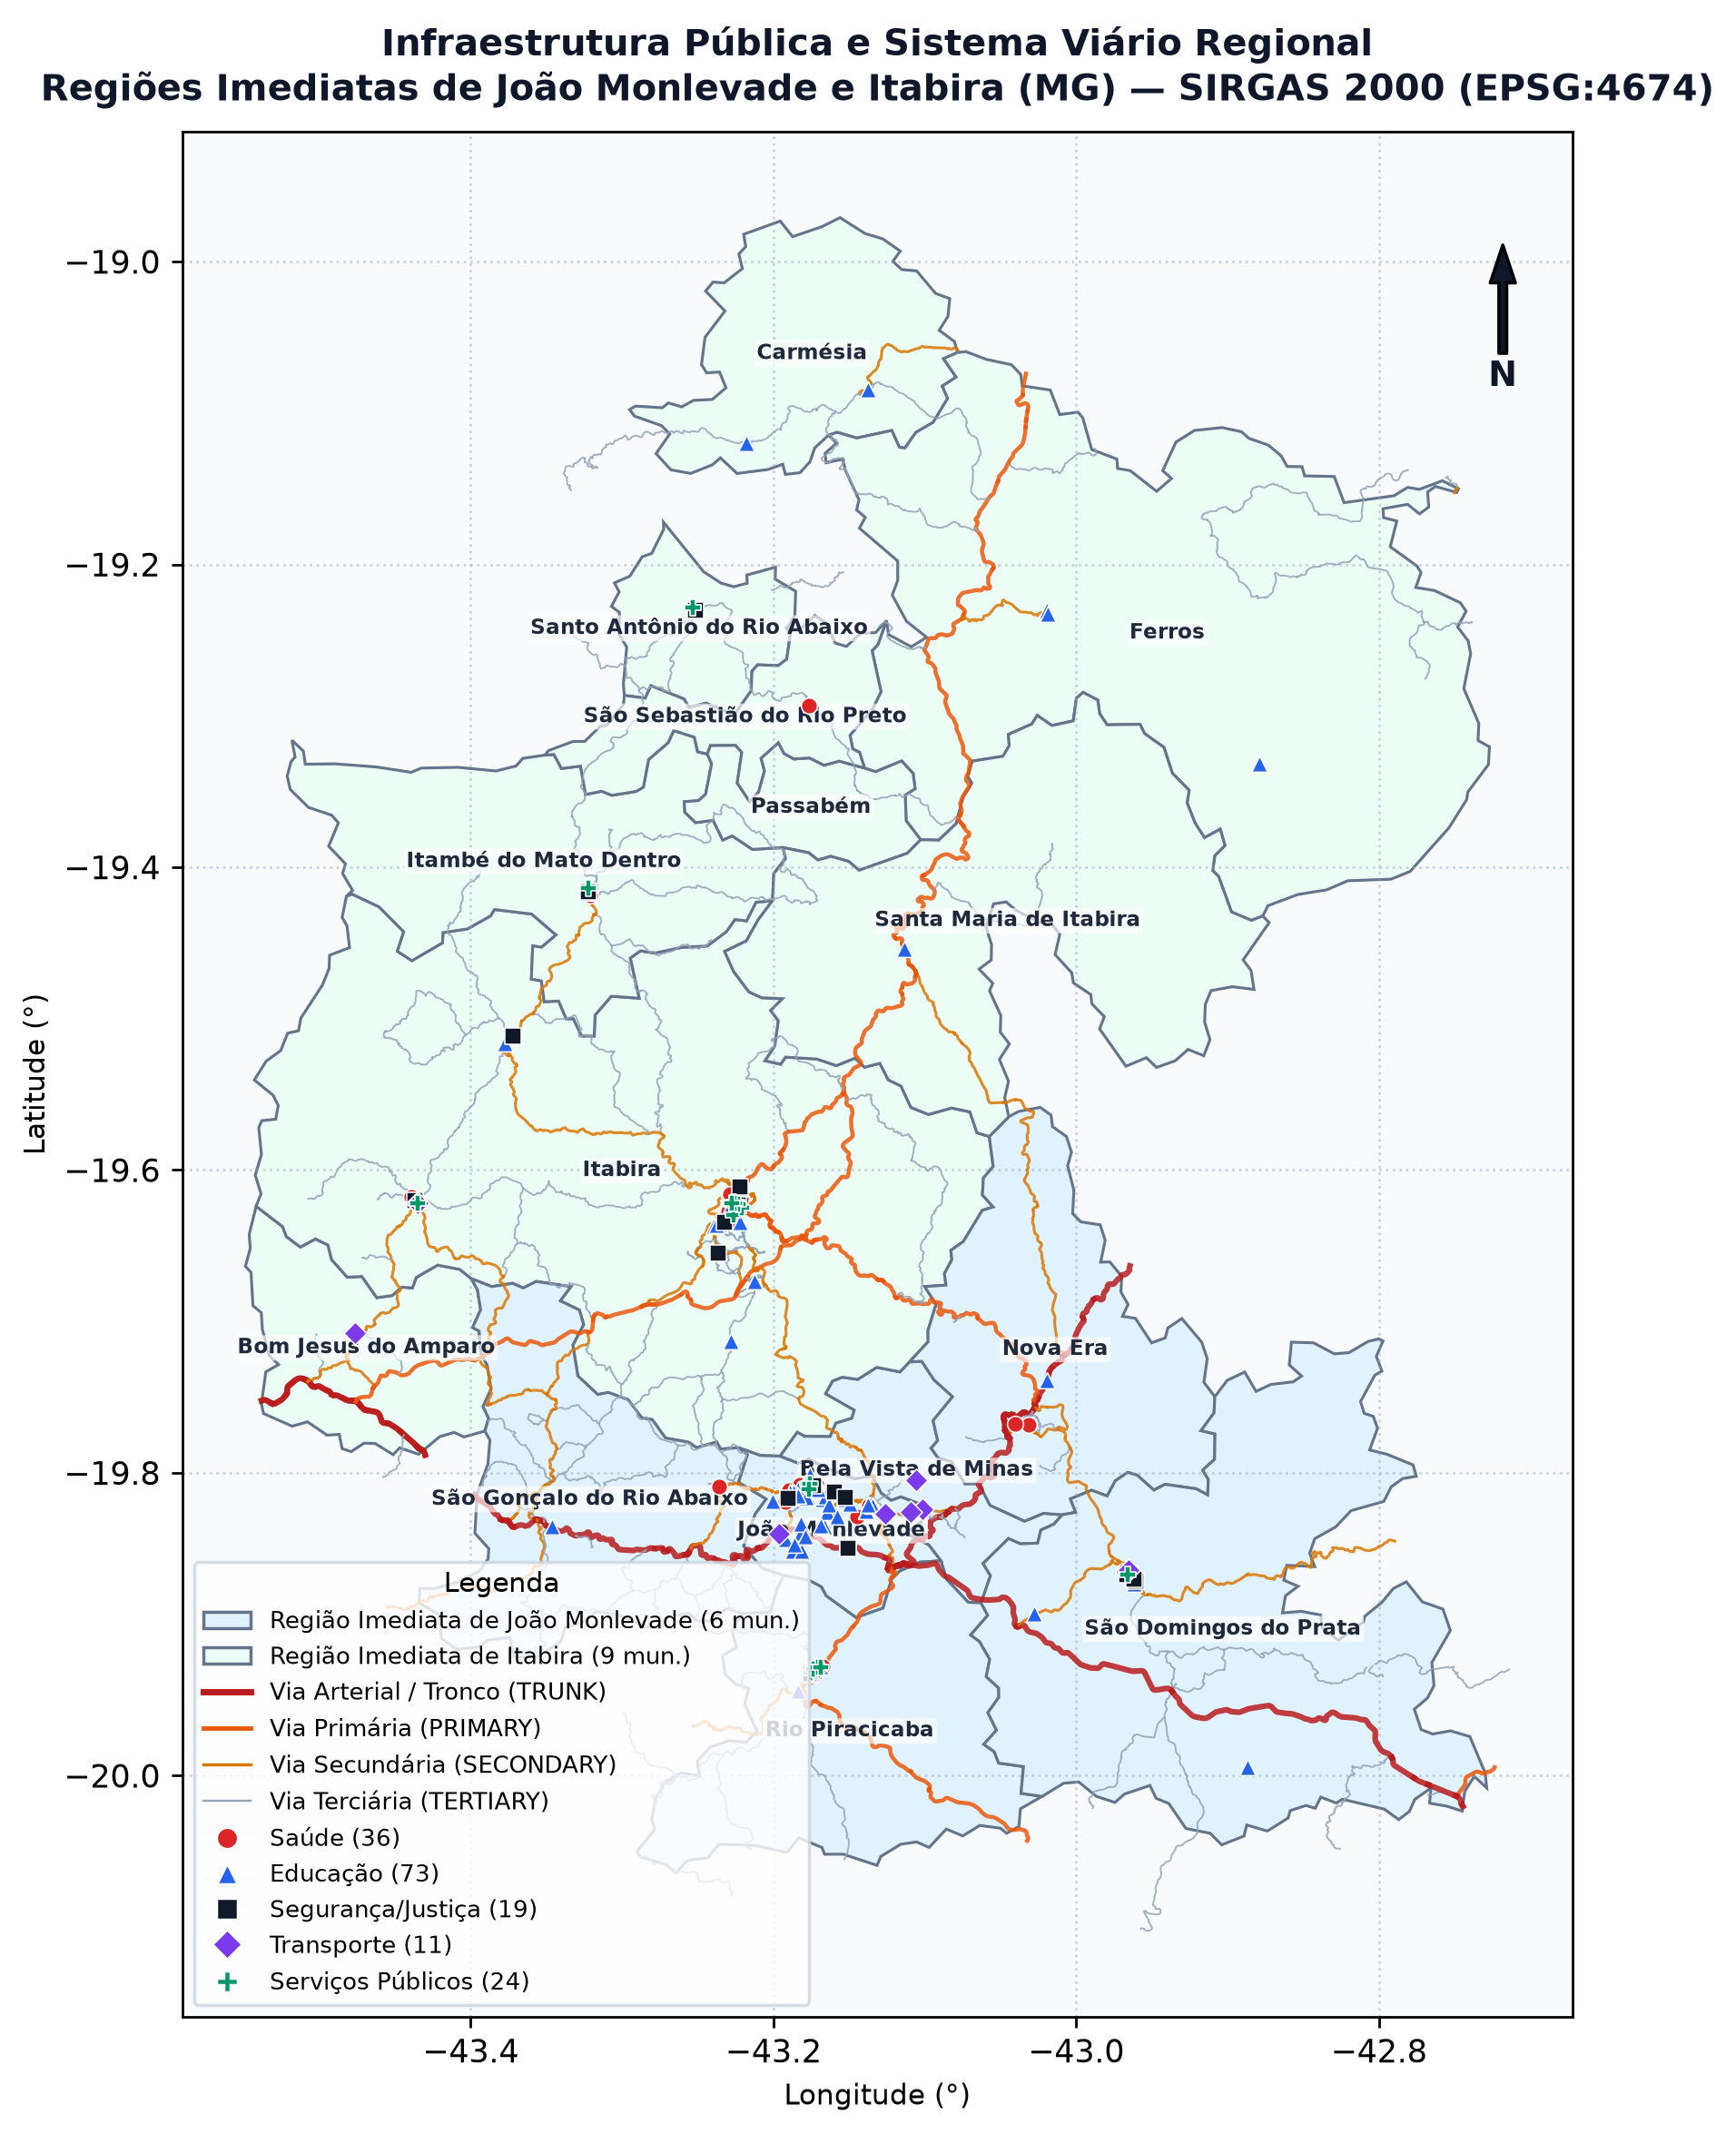
\includegraphics[width=0.92\textwidth]{mapa_recorte.png}
    \caption{Mapa da base geográfica: municípios, rede viária e equipamentos urbanos do recorte (EPSG:4674).}
    \label{fig:mapa_recorte}
\end{figure}

Sob o aspecto temporal, os limites municipais e dados demográficos correspondem ao retrato vigente do IBGE (Censo 2022), enquanto as feições viárias e de equipamentos urbanos refletem o estado colaborativo do OpenStreetMap na data da coleta (15/11/2026), não constituindo série histórica.

% ============================================================================
\chapter{Tratamento, Padronização e Validação}
% ============================================================================

Os dados brutos coletados passaram por um fluxo reprodutível de limpeza e padronização implementado em Python (\texttt{scripts/tratar\_dados.py}), utilizando as bibliotecas \texttt{shapely} e \texttt{pyproj}. Todas as métricas de filtragem e correção foram registradas em \texttt{scripts/log\_tratamento.txt}.

\section{Sistema de Referência Espacial (SRID)}

Adotou-se o sistema de referência \textbf{EPSG:4674 (SIRGAS 2000)} para todas as tabelas espaciais da base. A escolha justifica-se por ser o Sistema Geodésico de Referência oficial do Brasil e o datum nativo das malhas territoriais do IBGE, evitando distorções de reprojeção nos limites políticos. Como o EPSG:4674 utiliza coordenadas geográficas em graus, os cálculos métricos de área (\texttt{area\_km2}) e extensão (\texttt{extensao\_km}) durante o pré-processamento foram realizados mediante reprojeção temporária para \textbf{EPSG:31983 (SIRGAS 2000 / UTM zona 23S)}, correspondente à faixa longitudinal do recorte em Minas Gerais. Nas consultas em PostGIS, recomenda-se a conversão para o tipo \texttt{geography} ou transformação para \texttt{EPSG:31983}.

\section{Etapas de Limpeza e Filtragem}

\begin{enumerate}
    \item \textbf{Padronização geométrica e validade:} Conversão explícita de polígonos simples em \texttt{MultiPolygon} e de linhas simples em \texttt{MultiLineString}, assegurando uniformidade de tipo nas colunas do PostGIS. Todas as geometrias foram verificadas quanto à validade topológica (\texttt{is\_valid}) e não vacuidade (\texttt{not is\_empty}), sem necessidade de reparos estruturais nos dados finais.
    \item \textbf{Recorte espacial estrito:} A consulta à Overpass API utiliza uma caixa delimitadora (\emph{bounding box}) retangular, o que captura feições de municípios vizinhos fora da área de estudo. Realizou-se filtragem espacial exata contra a união dos 15 polígonos municipais:
    \begin{itemize}
        \item \emph{Equipamentos urbanos:} dos 256 elementos brutos, \textbf{163} permaneceram dentro dos limites municipais e \textbf{93} foram descartados por estarem fora do recorte.
        \item \emph{Trechos viários:} dos 3.026 elementos brutos, \textbf{2.001} intersectaram o recorte e \textbf{1.025} foram descartados.
    \end{itemize}
    \item \textbf{Atribuição de integridade referencial espacial:} Para cada equipamento urbano mantido, identificou-se o município continente por meio da relação topológica \texttt{contains}/\texttt{within}, preenchendo a chave estrangeira \texttt{cod\_ibge}.
    \item \textbf{Padronização textual e tratamento de nulos:} Nomes de tabelas e colunas foram definidos em \texttt{snake\_case} (minúsculas, sem acentos ou espaços), com codificação UTF-8. Nos 38 equipamentos que não possuíam a etiqueta \texttt{name} no OpenStreetMap, atribuiu-se um rótulo padronizado no formato \texttt{"<Tipo> sem nome (OSM <id>)"}.
\end{enumerate}

Ao final do processamento, a base consolidou \textbf{2.179 feições espaciais} (15 municípios, 163 equipamentos urbanos e 2.001 trechos viários) e 5 registros na tabela de domínio \texttt{categoria\_equipamento}.

% ============================================================================
\chapter{Modelagem e Estrutura no PostGIS}
% ============================================================================

O modelo relacional-espacial foi projetado para equilibrar normalização, integridade referencial e desempenho em consultas geográficas. A Figura~\ref{fig:der} ilustra o Diagrama Entidade-Relacionamento (DER) da base, destacando chaves primárias (PK), chaves estrangeiras (FK), restrições de unicidade (UQ), índices espaciais GiST e os relacionamentos espaciais documentados.

\begin{figure}[H]
    \centering
    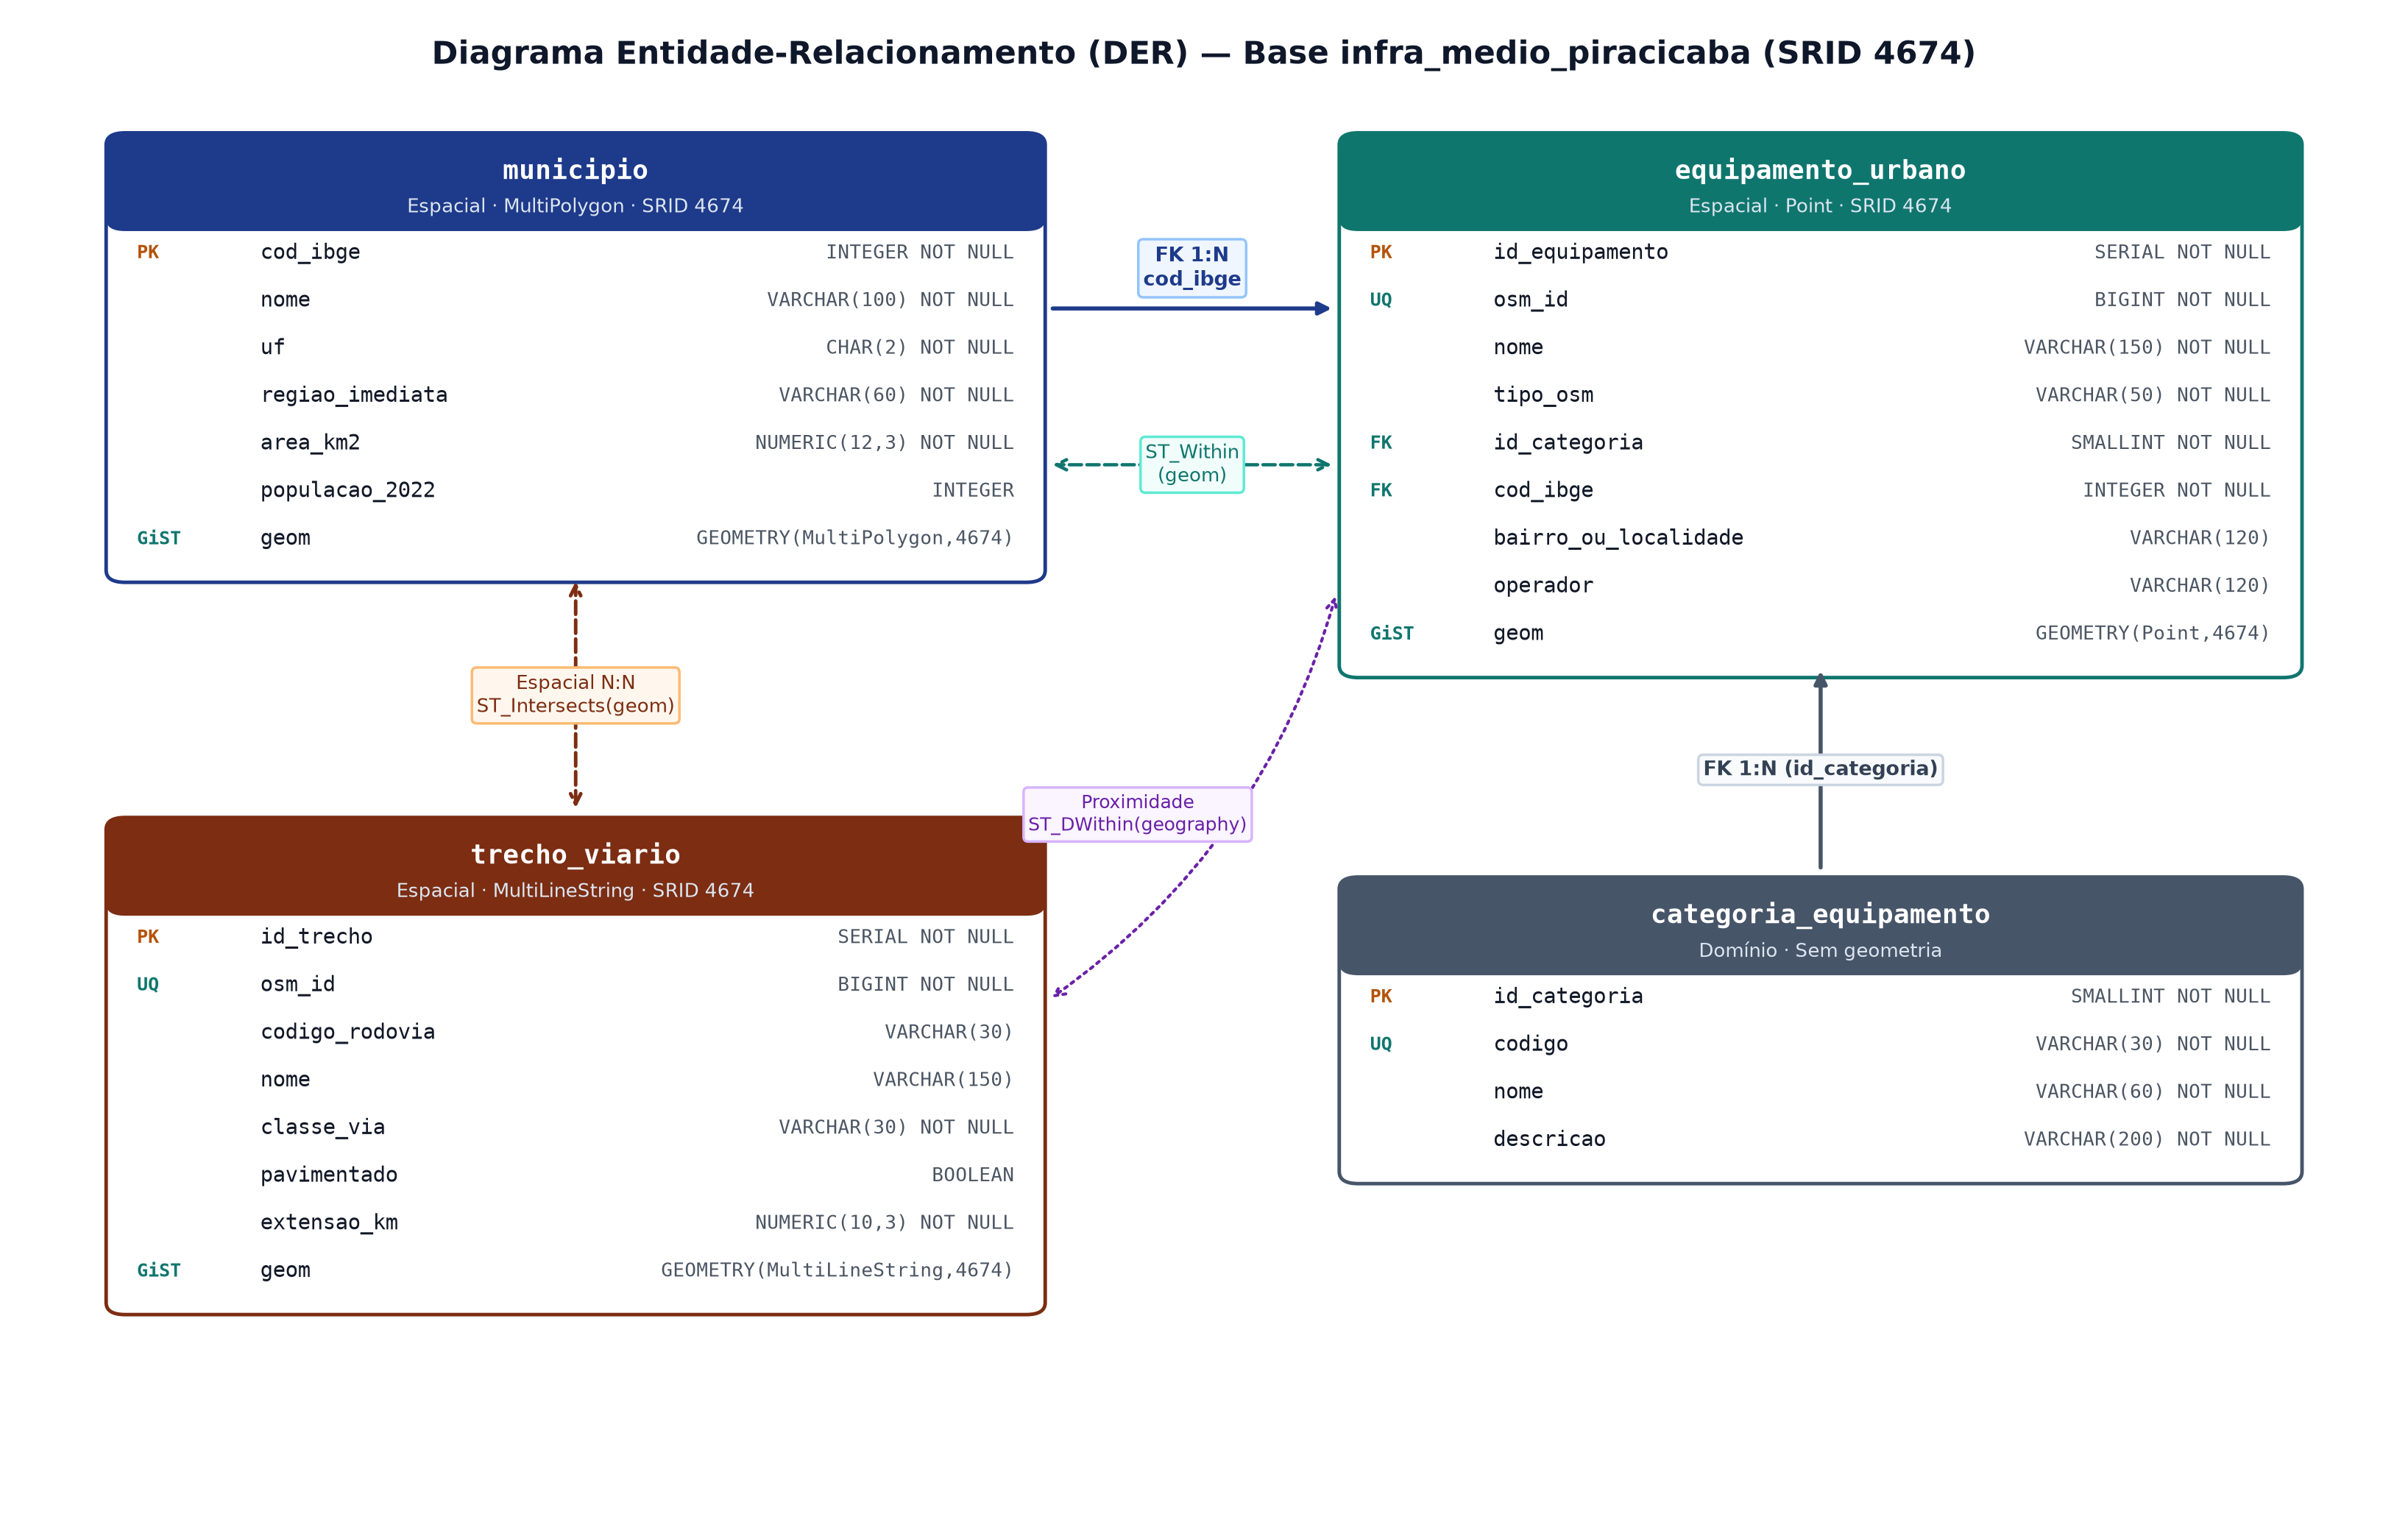
\includegraphics[width=0.98\textwidth]{der.png}
    \caption{Diagrama Entidade-Relacionamento (DER) da base \texttt{infra\_medio\_piracicaba}.}
    \label{fig:der}
\end{figure}

O script \texttt{sql/schema.sql} habilita a extensão \texttt{postgis}, cria as quatro tabelas com tipos geométricos tipados (\texttt{GEOMETRY(MultiPolygon, 4674)}, \texttt{GEOMETRY(Point, 4674)} e \texttt{GEOMETRY(MultiLineString, 4674)}), impõe restrições \texttt{CHECK} inclusive para validade geométrica (\texttt{ST\_IsValid(geom) AND NOT ST\_IsEmpty(geom)}) e cria índices espaciais GiST nas três tabelas geográficas, além de índices B-Tree auxiliares para chaves estrangeiras e filtros frequentes.

% ============================================================================
\chapter{Dicionário de Dados}
% ============================================================================

Este capítulo reproduz integralmente o conteúdo normativo do arquivo \texttt{DICIONARIO.md} do repositório.

\section{Visão Geral da Base}

\begin{table}[H]
\centering
\caption{Metadados gerais da base de dados geográficos.}
\label{tab:visao_geral}
\small
\begin{tabularx}{\textwidth}{>{\bfseries}p{4.0cm} X}
\toprule
Atributo & Descrição \\
\midrule
Título & Infraestrutura Pública e Sistema Viário Regional: Regiões Imediatas de João Monlevade e Itabira (\texttt{infra\_medio\_piracicaba}) \\
Finalidade & Apoiar análises de acessibilidade espacial, cobertura de serviços públicos e conectividade viária regional no PostGIS. \\
Fontes & IBGE (Localidades v1, Malhas v3 e Censo 2022) e OpenStreetMap (Overpass API). \\
Data de coleta & 15/11/2026 (todas as fontes). \\
Licença & IBGE (Dados Abertos -- Decreto 8.777/2016); OSM (ODbL 1.0); Código (MIT). \\
Cobertura espacial & 15 municípios de MG (6.099,38 km\textsuperscript{2}). \\
Cobertura temporal & Malha e Censo 2022 (IBGE); retrato OSM vigente em 15/11/2026. \\
SRID & EPSG:4674 (SIRGAS 2000). Cálculos métricos em EPSG:31983 ou \texttt{geography}. \\
Volume total & 2.179 feições espaciais + 5 registros de domínio. \\
\bottomrule
\end{tabularx}
\end{table}

\section{Descrição das Tabelas}

\subsection{Tabela \texttt{municipio}}
Limites territoriais oficiais e população residente dos municípios do recorte. \textbf{Geometria:} \texttt{MultiPolygon} $\cdot$ \textbf{SRID:} \texttt{4674} $\cdot$ \textbf{Registros:} \texttt{15}.

\begin{table}[H]
\centering
\caption{Estrutura da tabela \texttt{municipio}.}
\label{tab:municipio}
\scriptsize
\begin{tabularx}{\textwidth}{p{2.3cm} p{1.6cm} p{2.2cm} p{0.9cm} p{0.9cm} X p{2.1cm}}
\toprule
\textbf{Coluna} & \textbf{Tipo} & \textbf{Tam./Domínio} & \textbf{Nulo?} & \textbf{PK/FK} & \textbf{Descrição} & \textbf{Exemplo} \\
\midrule
\texttt{cod\_ibge} & \texttt{integer} & 7 dígitos & Não & PK & Código oficial do município no IBGE. & \texttt{3136207} \\
\texttt{nome} & \texttt{varchar} & 100 & Não & -- & Nome oficial do município em UTF-8. & João Monlevade \\
\texttt{uf} & \texttt{char} & 2 $\cdot$ \texttt{'MG'} & Não & -- & Sigla da unidade da federação. & \texttt{MG} \\
\texttt{regiao\_imediata} & \texttt{varchar} & 60 & Não & -- & Nome da Região Geográfica Imediata. & João Monlevade \\
\texttt{area\_km2} & \texttt{numeric} & (12,3) $\cdot$ $>$ 0 & Não & -- & Área territorial em km\textsuperscript{2} (EPSG:31983). & \texttt{98.519} \\
\texttt{populacao\_2022} & \texttt{integer} & $\ge$ 0 & Sim & -- & População residente (Censo 2022). & \texttt{80187} \\
\texttt{geom} & \texttt{geometry} & MultiPolygon, 4674 & Não & -- & Limite territorial do município. & \texttt{MULTIPOLYGON(...)} \\
\bottomrule
\end{tabularx}
\end{table}

\subsection{Tabela \texttt{categoria\_equipamento} (tabela de domínio)}
Classificação temática dos equipamentos urbanos. \textbf{Geometria:} Sem geometria $\cdot$ \textbf{Registros:} \texttt{5}.

\begin{table}[H]
\centering
\caption{Estrutura da tabela \texttt{categoria\_equipamento}.}
\label{tab:categoria}
\scriptsize
\begin{tabularx}{\textwidth}{p{2.3cm} p{1.6cm} p{2.2cm} p{0.9cm} p{0.9cm} X p{2.3cm}}
\toprule
\textbf{Coluna} & \textbf{Tipo} & \textbf{Tam./Domínio} & \textbf{Nulo?} & \textbf{PK/FK} & \textbf{Descrição} & \textbf{Exemplo} \\
\midrule
\texttt{id\_categoria} & \texttt{smallint} & 1 a 5 ($>$ 0) & Não & PK & Identificador numérico da categoria. & \texttt{1} \\
\texttt{codigo} & \texttt{varchar} & 30 $\cdot$ único & Não & -- & Código textual padronizado. & \texttt{SAUDE} \\
\texttt{nome} & \texttt{varchar} & 60 & Não & -- & Nome legível da categoria. & Saúde \\
\texttt{descricao} & \texttt{varchar} & 200 & Não & -- & Descrição dos tipos abrangidos. & Hospitais, clínicas... \\
\bottomrule
\end{tabularx}
\end{table}

\subsection{Tabela \texttt{equipamento\_urbano}}
Equipamentos públicos e comunitários georreferenciados. \textbf{Geometria:} \texttt{Point} $\cdot$ \textbf{SRID:} \texttt{4674} $\cdot$ \textbf{Registros:} \texttt{163}.

\begin{table}[H]
\centering
\caption{Estrutura da tabela \texttt{equipamento\_urbano}.}
\label{tab:equipamento}
\scriptsize
\begin{tabularx}{\textwidth}{p{2.6cm} p{1.4cm} p{2.1cm} p{0.9cm} p{0.9cm} X p{2.1cm}}
\toprule
\textbf{Coluna} & \textbf{Tipo} & \textbf{Tam./Domínio} & \textbf{Nulo?} & \textbf{PK/FK} & \textbf{Descrição} & \textbf{Exemplo} \\
\midrule
\texttt{id\_equipamento} & \texttt{serial} & gerado & Não & PK & Identificador sequencial interno. & \texttt{1} \\
\texttt{osm\_id} & \texttt{bigint} & único & Não & -- & Identificador original no OSM. & \texttt{1495738201} \\
\texttt{nome} & \texttt{varchar} & 150 & Não & -- & Nome do equipamento. & Hospital Margarida \\
\texttt{tipo\_osm} & \texttt{varchar} & 50 & Não & -- & Etiqueta \texttt{amenity} do OSM. & \texttt{hospital} \\
\texttt{id\_categoria} & \texttt{smallint} & ver domínio & Não & FK & Referencia \texttt{categoria\_equipamento}. & \texttt{1} \\
\texttt{cod\_ibge} & \texttt{integer} & 7 dígitos & Não & FK & Referencia \texttt{municipio.cod\_ibge}. & \texttt{3136207} \\
\texttt{bairro\_ou\_\allowbreak localidade} & \texttt{varchar} & 120 & Sim & -- & Bairro ou distrito informado. & Carneirinhos \\
\texttt{operador} & \texttt{varchar} & 120 & Sim & -- & Instituição mantenedora. & Prefeitura Municipal \\
\texttt{geom} & \texttt{geometry} & Point, 4674 & Não & -- & Localização pontual do equipamento. & \texttt{POINT(-43.17 -19.81)} \\
\bottomrule
\end{tabularx}
\end{table}

\subsection{Tabela \texttt{trecho\_viario}}
Trechos de rodovias federais, estaduais e vias estruturantes. \textbf{Geometria:} \texttt{MultiLineString} $\cdot$ \textbf{SRID:} \texttt{4674} $\cdot$ \textbf{Registros:} \texttt{2.001}.

\begin{table}[H]
\centering
\caption{Estrutura da tabela \texttt{trecho\_viario}.}
\label{tab:trecho}
\scriptsize
\begin{tabularx}{\textwidth}{p{2.3cm} p{1.4cm} p{2.3cm} p{0.9cm} p{0.9cm} X p{2.2cm}}
\toprule
\textbf{Coluna} & \textbf{Tipo} & \textbf{Tam./Domínio} & \textbf{Nulo?} & \textbf{PK/FK} & \textbf{Descrição} & \textbf{Exemplo} \\
\midrule
\texttt{id\_trecho} & \texttt{serial} & gerado & Não & PK & Identificador sequencial interno. & \texttt{1} \\
\texttt{osm\_id} & \texttt{bigint} & único & Não & -- & Identificador do \texttt{way} no OSM. & \texttt{28471930} \\
\texttt{codigo\_rodovia} & \texttt{varchar} & 30 & Sim & -- & Sigla oficial da rodovia (\texttt{ref}). & \texttt{BR-381} \\
\texttt{nome} & \texttt{varchar} & 150 & Sim & -- & Nome da via ou rodovia. & Av. Getúlio Vargas \\
\texttt{classe\_via} & \texttt{varchar} & 30 $\cdot$ CHECK & Não & -- & Hierarquia viária (\texttt{highway}). & \texttt{TRUNK} \\
\texttt{pavimentado} & \texttt{boolean} & T / F / NULL & Sim & -- & Indicador de pavimentação. & \texttt{TRUE} \\
\texttt{extensao\_km} & \texttt{numeric} & (10,3) $\cdot$ $\ge$ 0 & Não & -- & Extensão em km (EPSG:31983). & \texttt{1.425} \\
\texttt{geom} & \texttt{geometry} & MultiLineString, 4674 & Não & -- & Traçado geométrico do trecho. & \texttt{MULTILINESTRING(...)} \\
\bottomrule
\end{tabularx}
\end{table}

\section{Relacionamentos, Domínios e Limitações}

Os relacionamentos estruturais e espaciais são sumarizados na Tabela~\ref{tab:relacionamentos}. Quanto às limitações conhecidas, destaca-se que, por depender de mapeamento colaborativo no OpenStreetMap, municípios menores apresentam menor densidade de equipamentos cadastrados; além disso, 23,3\% dos equipamentos não possuíam tag \texttt{name} (recebendo rótulo padronizado), 57,1\% dos trechos viários não possuem \texttt{codigo\_rodovia} (vias urbanas) e 21,2\% não possuem informação de superfície (\texttt{pavimentado = NULL}).

\begin{table}[H]
\centering
\caption{Relacionamentos relacionais e espaciais da base.}
\label{tab:relacionamentos}
\scriptsize
\begin{tabularx}{\textwidth}{p{4.2cm} p{4.0cm} p{1.9cm} X}
\toprule
\textbf{Origem} & \textbf{Destino} & \textbf{Tipo} & \textbf{Descrição} \\
\midrule
\texttt{equipamento\_urbano.\allowbreak cod\_ibge} & \texttt{municipio.\allowbreak cod\_ibge} & FK 1:N & Cada equipamento pertence a um município. \\
\texttt{equipamento\_urbano.\allowbreak id\_categoria} & \texttt{categoria\_equipamento.\allowbreak id\_categoria} & FK 1:N & Cada equipamento possui uma categoria. \\
\texttt{equipamento\_urbano.\allowbreak geom} & \texttt{municipio.\allowbreak geom} & Espacial 1:N & \texttt{ST\_Within}: valida pertinência municipal. \\
\texttt{trecho\_viario.\allowbreak geom} & \texttt{municipio.\allowbreak geom} & Espacial N:N & \texttt{ST\_Intersects}: vias que cruzam municípios. \\
\texttt{equipamento\_urbano.\allowbreak geom} & \texttt{trecho\_viario.\allowbreak geom} & Espacial (dist.) & \texttt{ST\_DWithin(..., 500)} em \texttt{geography}. \\
\bottomrule
\end{tabularx}
\end{table}

% ============================================================================
\chapter{Consultas Espaciais e Reprodutibilidade}
% ============================================================================

O arquivo \texttt{sql/consultas.sql} disponibiliza seis consultas de validação e análise espacial, incluindo verificação de validade geométrica (\texttt{ST\_IsValid}), conferência de consistência entre chave estrangeira e \texttt{ST\_Within}, taxa de equipamentos por 10 mil habitantes, extensão viária por município via \texttt{ST\_Intersection} e análise de proximidade de unidades de saúde a rodovias principais:

\begin{lstlisting}[caption={Exemplo de consulta espacial de proximidade em PostGIS (\texttt{sql/consultas.sql}).}]
SELECT DISTINCT
       e.id_equipamento, e.nome AS equipamento, e.tipo_osm,
       m.nome AS municipio, t.codigo_rodovia,
       ROUND(ST_Distance(e.geom::geography, t.geom::geography)::NUMERIC, 1) AS distancia_m
FROM equipamento_urbano e
JOIN categoria_equipamento c ON c.id_categoria = e.id_categoria
JOIN municipio m ON m.cod_ibge = e.cod_ibge
JOIN trecho_viario t ON ST_DWithin(e.geom::geography, t.geom::geography, 500)
WHERE c.codigo = 'SAUDE'
  AND t.classe_via IN ('MOTORWAY', 'TRUNK', 'PRIMARY')
ORDER BY distancia_m ASC, e.nome;
\end{lstlisting}

Para importar a base em um banco PostgreSQL/PostGIS limpo (versões recomendadas: PostgreSQL 15+ e PostGIS 3.3+), basta executar em sequência:

\begin{verbatim}
createdb -U postgres -E UTF8 infra_medio_piracicaba
psql -U postgres -d infra_medio_piracicaba -v ON_ERROR_STOP=1 -f sql/schema.sql
psql -U postgres -d infra_medio_piracicaba -v ON_ERROR_STOP=1 -f sql/dados.sql
psql -U postgres -d infra_medio_piracicaba -v ON_ERROR_STOP=1 -f sql/consultas.sql
\end{verbatim}

% ============================================================================
\chapter{Considerações Finais}
% ============================================================================

O trabalho atingiu integralmente os objetivos propostos, consolidando uma base de dados geográficos vetoriais com 2.179 feições espaciais distribuídas em três tipos geométricos (\texttt{MultiPolygon}, \texttt{MultiLineString} e \texttt{Point}) e quatro tabelas relacionadas no modelo relacional-espacial do PostGIS. A automação da coleta e do tratamento em Python assegura reprodutibilidade completa, enquanto o dicionário de dados em Markdown e o presente relatório técnico fornecem transparência quanto às fontes, licenças, escolhas de projeção e limitações inerentes aos dados colaborativos.

% ============================================================================
\begin{thebibliography}{9}

\bibitem{ibge2022}
INSTITUTO BRASILEIRO DE GEOGRAFIA E ESTATÍSTICA (IBGE). \textbf{API de Serviços de Dados: Localidades, Malhas Territoriais e Agregados (Censo Demográfico 2022)}. Rio de Janeiro: IBGE, 2026. Disponível em: \url{https://servicodados.ibge.gov.br/api/docs}. Acesso em: 15 nov. 2026.

\bibitem{osm2026}
OPENSTREETMAP CONTRIBUTORS. \textbf{OpenStreetMap Database / Overpass API}. Cambridge: OpenStreetMap Foundation, 2026. Licença ODbL 1.0. Disponível em: \url{https://www.openstreetmap.org}. Acesso em: 15 nov. 2026.

\bibitem{postgis2025}
POSTGIS PROJECT STEERING COMMITTEE. \textbf{PostGIS 3.4/3.5 Manual}. 2025. Disponível em: \url{https://postgis.net/documentation/}. Acesso em: 15 nov. 2026.

\bibitem{brasil2016}
BRASIL. Decreto nº 8.777, de 11 de maio de 2016. Institui a Política de Dados Abertos do Poder Executivo federal. \textbf{Diário Oficial da União}, Brasília, DF, 12 maio 2016.

\end{thebibliography}

\end{document}
